%FIXME: check if %>>% is actually copyable
%FIXME: use hidden linebreaks in copyable code?
\documentclass{beamer}

\usepackage[orientation=landscape,size=a0,scale=1.4,debug]{beamerposter}
\mode<presentation>{\usetheme{mlr}}

\usepackage[sfdefault]{roboto}
\usepackage{roboto-mono}
\usepackage[T1]{fontenc}
\usepackage[utf8]{inputenc} % UTF-8
\usepackage[english]{babel} % Language
\usepackage{hyperref} % Hyperlinks
\usepackage{ragged2e} % Text position
\usepackage[export]{adjustbox} % Image position
\usepackage[most]{tcolorbox} % Code boxes

\hypersetup{
    hyperfootnotes=false,
    colorlinks=true,
	linktocpage=true,
	pdfauthor={mlr-org team},
    %linkcolor=[RGB]{3,99,142}, % mlr blue
    urlcolor=[RGB]{231,138,69}
}

\title{Dataflow programming with mlr3pipelines :\,: CHEAT SHEET} % Package title in header, \, adds thin space between ::

\newlength{\columnheight} % Adjust depending on header height
\setlength{\columnheight}{84cm} 

\newtcolorbox{codebox}{%
	sharp corners,
	leftrule=0pt,
	rightrule=0pt,
	toprule=0pt,
	bottomrule=0pt,
	hbox}

\newtcolorbox{codeboxmultiline}[1][]{%
	sharp corners,
	leftrule=0pt,
	rightrule=0pt,
	toprule=0pt,
	bottomrule=0pt,
	#1}

\newtcolorbox{codeboxexample}{%
	sharp corners,
	leftrule=0pt,
	rightrule=0pt,
	toprule=0pt,
	bottomrule=0pt,
	fontupper=\robotomono\small,
	width=27cm,
	adjusted title=Example,
	fonttitle = \bfseries\Large,
	top = 0.5em}

\newtcolorbox{codeboxinline}{%
	sharp corners,
	leftrule=0pt,
	rightrule=0pt,
	toprule=0pt,
	bottomrule=0pt,
	hbox,
	nobeforeafter,
	tcbox raise base}

\newcommand{\codeinline}[1]{\begin{codeboxinline}#1\end{codeboxinline}}

\begin{document}
\begin{frame}[fragile]{}
	\begin{columns}
		\begin{column}{.245\textwidth}
			\begin{beamercolorbox}[center]{postercolumn}
				\begin{minipage}{.98\textwidth}
					\parbox[t][\columnheight]{\textwidth}{
						\begin{myblock}{Intro}
              The mlr3pipelines package is an extension for the \href{https://github.com/mlr-org/mlr3}{mlr3} package and provides \codeinline{PipeOp}s (pipeline operators) which can be connected to a \codeinline{Graph}.
            \end{myblock}
						\begin{myblock}{PipeOps}
              A \codeinline{PipeOp} represents transformative operations on its input leading to its output but behaves differently during ``training'' and ``prediction''. During training, the \codeinline{PipeOp} stores the transformation appied to the training data. This information is then used during the prediction.\\
              \ \\
              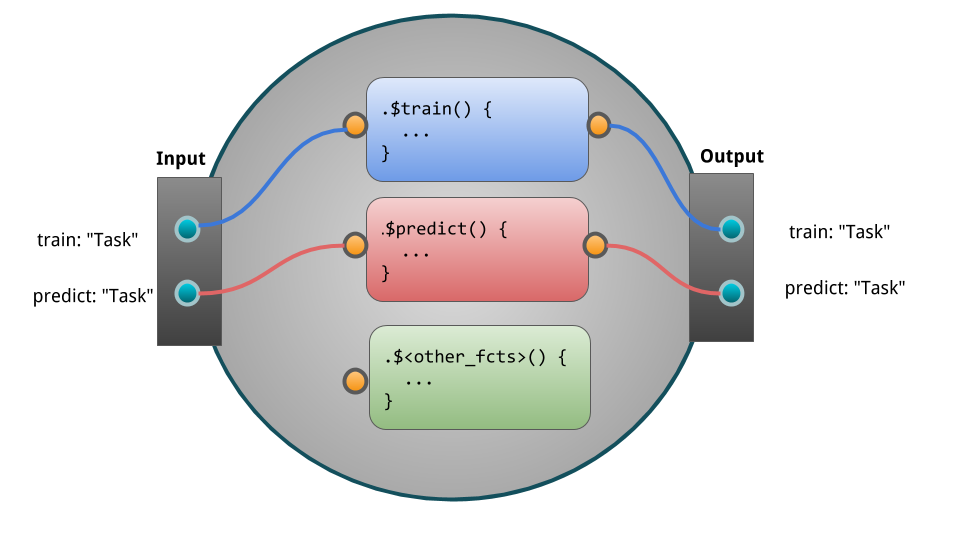
\includegraphics[width=\textwidth]{img/po_viz.png}
              Important \codeinline{PipeOp}s:
              \begin{itemize}
                \item Data Transformer: \codeinline{PipeOpPCA}
                \item Feature Selection: \codeinline{PipeOpFilter}
                \item Repair Tasks: \codeinline{PipeOpRemoveConstants}
                \item Factor Encoding: \codeinline{PipeOpEncode}
                \item Imbalanced Data: \codeinline{PipeOpClassBalancing}
                \item Missing Data: \codeinline{PipeOpImputeHist}
                \item Any Learner: \codeinline{PipeOpLearner}
                \item Ensembles: \codeinline{PipeOpLearnerCV}
              \end{itemize}
              \ \\
              Full list: \codeinline{as.data.table(mlr\_pipeops)}\\
              \ \\
              Construction via a \codeinline{.key}, e.g.: \codeinline{pca = \textbf{po}("pca")}\\
              \ \\
              Important methods and slots:
              \begin{itemize}
                \item \codeinline{\$\textbf{train}()} %takes a list of input arguments and turns them into a list of outputs while saving a state.
                \item \codeinline{\$\textbf{predict}()} %takes a list of input arguments and turns them into a list of outputs relying on the saved state.
                \item \codeinline{\$\textbf{state}} %contains the trained ``model'' wich is utilized during predicton
              \end{itemize}
						\end{myblock}
						\vfill}
				\end{minipage}
			\end{beamercolorbox}
		\end{column}
		\begin{column}{.245\textwidth}
			\begin{beamercolorbox}[center]{postercolumn}
				\begin{minipage}{.98\textwidth}
					\parbox[t][\columnheight]{\textwidth}{
						\begin{myblock}{Graphs}
              A \codeinline{Graph} connects \codeinline{PipeOp}s with edges mandating how data should be flowing along them. A \codeinline{Graph} itself has a \codeinline{\$train()} and \codeinline{\$predict()} method that accept data and propagate this data through the network of \codeinline{PipeOp}s. The return value corresponds to the output of the \codeinline{PipeOp} outputs that are not connected to other \codeinline{PipeOp}s.\\
              \ \\
              %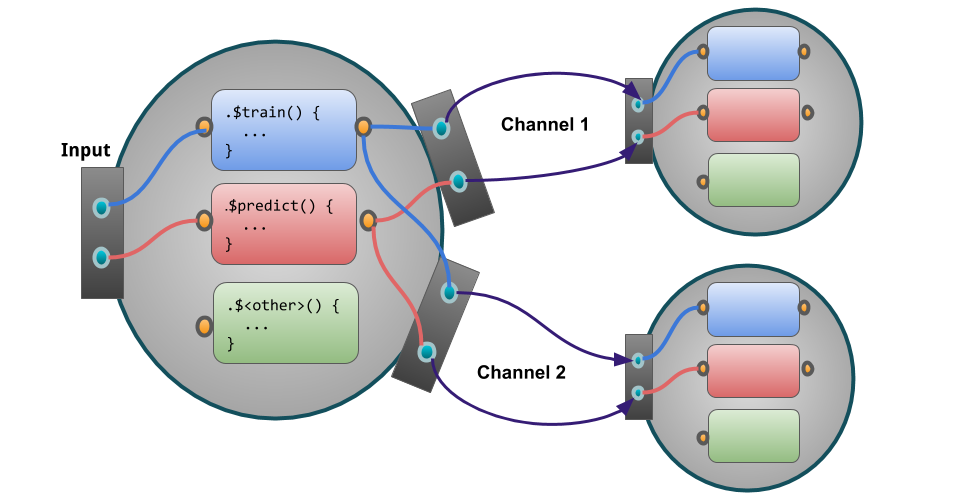
\includegraphics[width=\textwidth]{img/po_multi_viz.png}
              The \codeinline{\%>>\%} operator takes either a \codeinline{PipeOp} or a \codeinline{Graph} on each of its sides and connects all left-hand outputs to the right-hand inputs:
              \begin{codebox}
                gr = po("pca") \textbf{\%>>\%} lrn("classif.rpart")
              \end{codebox}
              \ \\
              Printing and plotting the \codeinline{Graph}:
              \begin{codeboxmultiline}[width=13cm]
                \textbf{print}(gr)\\
                gr\$\textbf{plot}(html = TRUE)
              \end{codeboxmultiline}
              \ \\
              %Assessing the \codeinline{PipeOp}s: \codeinline{gr\$\textbf{pipeops}}\\
              %\ \\
              To have full control over the edges, construct an empty \codeinline{Graph}, add \codeinline{PipeOp}s and connect them manually via their \codeinline{\$id}:
              \begin{codeboxmultiline}[width=20cm]
                gr = \textbf{Graph}\$new()\\
                gr\$\textbf{add\_pipeop}(po("pca"))\\
                gr\$\textbf{add\_pipeop}(lrn("classif.rpart"))
                gr\$\textbf{add\_edge}("pca", "classif.rpart")
              \end{codeboxmultiline}
						\end{myblock}
            \begin{myblock}{Learners and Graphs}
              Any \codeinline{Learner} can be wrapped in a \codeinline{PipeOp}, more precisely a \codeinline{PipeOpLearner}, e.g.:
              \begin{codebox}
                po(lrn("classif.rpart"))
              \end{codebox}
              \ \\
              Analogously, any \codeinline{Graph} can be wrappend in a \codeinline{Learner}, resulting in a \codeinline{GraphLearner}:
              \begin{codebox}
                grl = GraphLearner\$new(gr)
              \end{codebox}
              \ \\
              When predicting from a \codeinline{Graph} you have to set the predict type of the \codeinline{GraphLearner} explicitly, i.e.:
              \begin{codebox}
                grl\$predict\_type = "prob"
              \end{codebox}
            \end{myblock}
						\vfill}
				\end{minipage}
			\end{beamercolorbox}
		\end{column}
		\begin{column}{.245\textwidth}
			\begin{beamercolorbox}[center]{postercolumn}
				\begin{minipage}{.98\textwidth}
					\parbox[t][\columnheight]{\textwidth}{
            \begin{myblock}{Nonlinear Graphs}
              \codeinline{\textbf{gunion}()} arranges \codeinline{PipeOp}s or \codeinline{Graph}s next to each other in a disjoint graph union. \\
              \ \\
              This allows for splitting a node into several paths, i.e., \textbf{branching} (where only one path will be executed):
              \begin{codeboxexample}
						    {\footnotesize
                  choices = c("pca", "scale")\\
                  gr = po("branch", options = choices) \%>>\%\\
                  \hspace*{1ex} gunion(list(po("pca"), po("scale"))) \%>>\%\\
                  \hspace*{1ex} po("unbranch", options = choices)\\
                  gr\$plot(html = TRUE)\\
                  \ \\
                  \# set the "pca" path active:
                  gr\$param\_set\$values\$branch.selection = "pca"}
					      \end{codeboxexample}
              \ \\
              \codeinline{PipeOpFeatureUnion} aggregates features from all input tasks into a single \codeinline{Task}:
              \begin{codeboxexample}
						    {\footnotesize
                  task = tsk("iris")\\
                  gr = gunion(list(po("nop"), po("pca"))) \%>>\%\\
                  \hspace*{1ex} po("featureunion")\\
                  gr\$train(task)}
              \end{codeboxexample}
              \ \\
              \codeinline{\textbf{greplicate}()} creates a new \codeinline{Graph} containing \codeinline{n} copies of the input (\codeinline{PipeOp} or \codeinline{Graph}). \\
              \ \\
              Together with \codeinline{PipeOpSubsample} this straightforward allows for \textbf{bagging}:
              \begin{codeboxexample}
						    {\footnotesize
                  pr = po("subsample") \%>>\% lrn("classif.rpart") \\
                  bagging = greplicate(pr, n = 10) \%>>\%\\
                  \hspace*{1ex} po("classifavg", innum = 10)\\
                  bagging\$plot(html = TRUE)}
					    \end{codeboxexample}
            \end{myblock}
						\vfill}
				\end{minipage}
			\end{beamercolorbox}
		\end{column}
    \begin{column}{.245\textwidth}
			\begin{beamercolorbox}[center]{postercolumn}
				\begin{minipage}{.98\textwidth}
					\parbox[t][\columnheight]{\textwidth}{
            \begin{myblock}{Hyperparameters}
              mlr3pipelines relies on the paradox package to provide parameters that can modify a \codeinline{PipeOp}'s behavior. To inspect the parameters see the \codeinline{\$param\_set}, e.g., \codeinline{po("pca")\$\textbf{param\_set}}\\
              \ \\
              Access the \codeinline{\$param\_set\$values} slot to set or retrieve a parameter, or specify \codeinline{param\_vals} during construction:
              \begin{codeboxmultiline}[width=25cm]
                pca = po("pca") \\
                pca\$param\_set\$\textbf{values} = list(scale = TRUE) \\
                po("pca", \textbf{param\_vals} = list(scale = TRUE)
              \end{codeboxmultiline}
              \ \\
              In a \codeinline{Graph}, the parameters of all \codeinline{PipeOp}s are collected. Both \codeinline{PipeOpLearner} and \codeinline{GraphLearner} preserve parameters of the objects they encapsulate.
            \end{myblock}
            \begin{myblock}{Tuning}
              Construct a \codeinline{TuningInstance} consisting of a \codeinline{Task}, \codeinline{Learner}, \codeinline{Resampling} method, \codeinline{ParamSet} for the hyperparameters, \codeinline{Measure} as a performance evaluator, and a \codeinline{Terminator} as a stop criterion (see also \href{FIXME:CheatsheetLink}{mlr3tuning}):
              \begin{codeboxexample}
						  {\footnotesize
                task = tsk("iris")\\
                gr = po("pca") \%»\% lrn("classif.rpart")\\
                grl = GraphLearner\$new(gr)\\
                \ \\
                ps\_tune = ParamSet\$new(list(\\
                \hspace*{1ex} ParamDbl\$new("classif.rpart.cp",\\
                \hspace*{2ex} lower = 0, upper = 0.05)\\
                ))\\
                \ \\
                instance = TuningInstance\$new(\\
                \hspace*{1ex} task = task,\\
                \hspace*{1ex} learner = grl,\\
                \hspace*{1ex} resampling = rsmp("holdout"),\\
                \hspace*{1ex} measures = msr("classif.ce"),\\
                \hspace*{1ex} param\_set = ps\_tune,\\
                \hspace*{1ex} terminator = term("evals", n\_evals = 10)\\
                ) \\
                \ \\
                tuner = TunerRandomSearch\$new()\\
                tuner\$tune(instance)\\
                instance\$result}
					    \end{codeboxexample}
            \end{myblock}
						\vfill}
				\end{minipage}
			\end{beamercolorbox}
		\end{column}
	\end{columns}
\end{frame}
\end{document}
